\section{DIL\_\-Visualize\_\-with\_\-FORM\_\-Tabs  Class Reference}
\label{classDIL__Visualize__with__FORM__Tabs}\index{DIL_Visualize_with_FORM_Tabs@{DIL\_\-Visualize\_\-with\_\-FORM\_\-Tabs}}
{\tt \#include $<$dil2al.hh$>$}

Inheritance diagram for DIL\_\-Visualize\_\-with\_\-FORM\_\-Tabs::\begin{figure}[H]
\begin{center}
\leavevmode
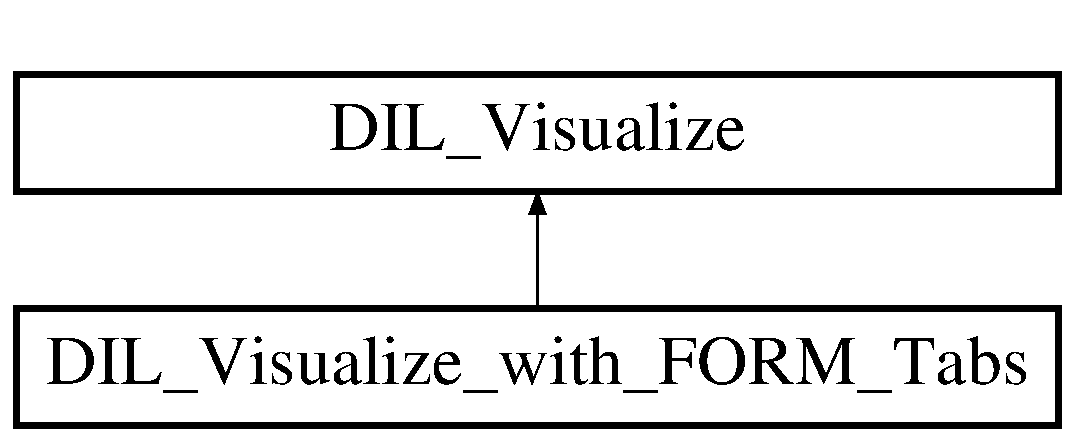
\includegraphics[height=2cm]{classDIL__Visualize__with__FORM__Tabs}
\end{center}
\end{figure}
\subsection*{Public Methods}
\begin{CompactItemize}
\item 
{\bf DIL\_\-Visualize\_\-with\_\-FORM\_\-Tabs} ({\bf DIL\_\-Hierarchy\_\-Level\_\-Data} $\ast$ld=NULL)
\item 
virtual void {\bf Initialize} ()
\item 
virtual void {\bf Visualize\_\-Element} ({\bf DIL\_\-entry} $\ast$de, int depth)
\item 
virtual void {\bf Visualize\_\-Not\-Shown} (int numdependencies, int depth)
\item 
virtual {\bf String} {\bf Output} ()
\item 
virtual {\bf String} {\bf Output\_\-Content} ()
\item 
virtual void {\bf Append} ({\bf String} appendstr)
\end{CompactItemize}
\subsection*{Protected Methods}
\begin{CompactItemize}
\item 
virtual bool {\bf Visualize\_\-Plan\_\-Entry} ({\bf DIL\_\-entry} $\ast$de)
\end{CompactItemize}
\subsection*{Protected Attributes}
\begin{CompactItemize}
\item 
{\bf String} {\bf s}
\item 
{\bf String} {\bf content}
\end{CompactItemize}


\subsection{Constructor \& Destructor Documentation}
\index{DIL_Visualize_with_FORM_Tabs@{DIL\_\-Visualize\_\-with\_\-FORM\_\-Tabs}!DIL_Visualize_with_FORM_Tabs@{DIL\_\-Visualize\_\-with\_\-FORM\_\-Tabs}}
\index{DIL_Visualize_with_FORM_Tabs@{DIL\_\-Visualize\_\-with\_\-FORM\_\-Tabs}!DIL_Visualize_with_FORM_Tabs@{DIL\_\-Visualize\_\-with\_\-FORM\_\-Tabs}}
\subsubsection{\setlength{\rightskip}{0pt plus 5cm}DIL\_\-Visualize\_\-with\_\-FORM\_\-Tabs::DIL\_\-Visualize\_\-with\_\-FORM\_\-Tabs ({\bf DIL\_\-Hierarchy\_\-Level\_\-Data} $\ast$ {\em ld} = NULL)\hspace{0.3cm}{\tt  [inline]}}\label{classDIL__Visualize__with__FORM__Tabs_a0}




Definition at line 795 of file dil2al.hh.



\footnotesize\begin{verbatim}795 : DIL_Visualize(ld) {}
\end{verbatim}\normalsize 


\subsection{Member Function Documentation}
\index{DIL_Visualize_with_FORM_Tabs@{DIL\_\-Visualize\_\-with\_\-FORM\_\-Tabs}!Append@{Append}}
\index{Append@{Append}!DIL_Visualize_with_FORM_Tabs@{DIL\_\-Visualize\_\-with\_\-FORM\_\-Tabs}}
\subsubsection{\setlength{\rightskip}{0pt plus 5cm}virtual void DIL\_\-Visualize\_\-with\_\-FORM\_\-Tabs::Append ({\bf String} {\em appendstr})\hspace{0.3cm}{\tt  [inline, virtual]}}\label{classDIL__Visualize__with__FORM__Tabs_a6}




Definition at line 801 of file dil2al.hh.

Referenced by Tabbed\_\-FORM\_\-DIL\_\-Hierarchy().



\footnotesize\begin{verbatim}801 { s += appendstr; }
\end{verbatim}\normalsize 
\index{DIL_Visualize_with_FORM_Tabs@{DIL\_\-Visualize\_\-with\_\-FORM\_\-Tabs}!Initialize@{Initialize}}
\index{Initialize@{Initialize}!DIL_Visualize_with_FORM_Tabs@{DIL\_\-Visualize\_\-with\_\-FORM\_\-Tabs}}
\subsubsection{\setlength{\rightskip}{0pt plus 5cm}virtual void DIL\_\-Visualize\_\-with\_\-FORM\_\-Tabs::Initialize ()\hspace{0.3cm}{\tt  [inline, virtual]}}\label{classDIL__Visualize__with__FORM__Tabs_a1}




Reimplemented from {\bf DIL\_\-Visualize} {\rm (p.\,\pageref{classDIL__Visualize_a1})}.

Definition at line 796 of file dil2al.hh.



\footnotesize\begin{verbatim}796 { s = ""; content = ""; }
\end{verbatim}\normalsize 
\index{DIL_Visualize_with_FORM_Tabs@{DIL\_\-Visualize\_\-with\_\-FORM\_\-Tabs}!Output@{Output}}
\index{Output@{Output}!DIL_Visualize_with_FORM_Tabs@{DIL\_\-Visualize\_\-with\_\-FORM\_\-Tabs}}
\subsubsection{\setlength{\rightskip}{0pt plus 5cm}virtual {\bf String} DIL\_\-Visualize\_\-with\_\-FORM\_\-Tabs::Output ()\hspace{0.3cm}{\tt  [inline, virtual]}}\label{classDIL__Visualize__with__FORM__Tabs_a4}




Reimplemented from {\bf DIL\_\-Visualize} {\rm (p.\,\pageref{classDIL__Visualize_a7})}.

Definition at line 799 of file dil2al.hh.

Referenced by Tabbed\_\-FORM\_\-DIL\_\-Hierarchy().



\footnotesize\begin{verbatim}799 { return s; }
\end{verbatim}\normalsize 
\index{DIL_Visualize_with_FORM_Tabs@{DIL\_\-Visualize\_\-with\_\-FORM\_\-Tabs}!Output_Content@{Output\_\-Content}}
\index{Output_Content@{Output\_\-Content}!DIL_Visualize_with_FORM_Tabs@{DIL\_\-Visualize\_\-with\_\-FORM\_\-Tabs}}
\subsubsection{\setlength{\rightskip}{0pt plus 5cm}virtual {\bf String} DIL\_\-Visualize\_\-with\_\-FORM\_\-Tabs::Output\_\-Content ()\hspace{0.3cm}{\tt  [inline, virtual]}}\label{classDIL__Visualize__with__FORM__Tabs_a5}




Definition at line 800 of file dil2al.hh.

Referenced by Tabbed\_\-FORM\_\-DIL\_\-Hierarchy().



\footnotesize\begin{verbatim}800 { return content; }
\end{verbatim}\normalsize 
\index{DIL_Visualize_with_FORM_Tabs@{DIL\_\-Visualize\_\-with\_\-FORM\_\-Tabs}!Visualize_Element@{Visualize\_\-Element}}
\index{Visualize_Element@{Visualize\_\-Element}!DIL_Visualize_with_FORM_Tabs@{DIL\_\-Visualize\_\-with\_\-FORM\_\-Tabs}}
\subsubsection{\setlength{\rightskip}{0pt plus 5cm}void DIL\_\-Visualize\_\-with\_\-FORM\_\-Tabs::Visualize\_\-Element ({\bf DIL\_\-entry} $\ast$ {\em de}, int {\em depth})\hspace{0.3cm}{\tt  [virtual]}}\label{classDIL__Visualize__with__FORM__Tabs_a2}




Reimplemented from {\bf DIL\_\-Visualize} {\rm (p.\,\pageref{classDIL__Visualize_a5})}.

Definition at line 187 of file diladmin.cc.

References DIL\_\-ID::chars(), DIL\_\-entry\_\-content::completion, DIL\_\-entry::content, content, DIL\_\-Visualize::cumlikelihood, DIL\_\-Topical\_\-List::dil, Elipsis\_\-At(), DIL\_\-entry::Entry\_\-Text(), filetitle\_\-t::file, String::gsub(), HTML\_\-put\_\-href(), HTML\_\-remove\_\-tags(), DIL\_\-Visualize::Level\_\-Data(), replicate(), s, DIL\_\-ID::str(), DIL\_\-entry::Topics(), and Visualize\_\-Plan\_\-Entry().



\footnotesize\begin{verbatim}187                                                                               {
188   String ptxtcontent;
189   content += "\nDIL#" + String(de->chars()) + ":\n";
190   String * ctxt = de->Entry_Text();
191   if (ctxt) {
192     ptxtcontent = (*ctxt);
193     content += (*HTML_remove_tags(ptxtcontent));
194     Elipsis_At(ptxtcontent,hierarchyexcerptlength);
195     ptxtcontent.gsub('\n',' ');
196   } else ptxtcontent = "<!-- excerpt requires content file option -->";
197   content += '\n';
198   if (depth>0) s += replicate('\t',depth);
199   else cumlikelihood = 0.0;
200   // differentiation of display depending on completion status
201   bool pending = true;
202   if (de->content) pending = ((de->content->completion>=0.0) && (de->content->completion<1.0));
203   // show checkbox and DIL ID reference
204   s += "<INPUT type=\"checkbox\" name=\"DILIDCHKBX"+String(de->chars())+"\" value=\"extract\">";
205   if (pending) s += HTML_put_href((de->Topics(0)->dil.file+'#')+de->chars(),"<B>DIL#" + String(de->chars()) + "</B>");
206   else s += HTML_put_href((de->Topics(0)->dil.file+'#')+de->chars(),"DIL#" + String(de->chars()));
207   // show level-specific data
208   if (Level_Data()) { // visualization that depends on level-specific data
209     if (!Visualize_Plan_Entry(de)) if (de->content) s += "[<A HREF=\"file:///cgi-bin/dil2al?dil2al=MEI&DILID="+de->str()+"\">edit</A>]";
210   }
211   // show DIL entry text content
212   s += ": " + ptxtcontent + '\n';
213 }
\end{verbatim}\normalsize 
\index{DIL_Visualize_with_FORM_Tabs@{DIL\_\-Visualize\_\-with\_\-FORM\_\-Tabs}!Visualize_NotShown@{Visualize\_\-NotShown}}
\index{Visualize_NotShown@{Visualize\_\-NotShown}!DIL_Visualize_with_FORM_Tabs@{DIL\_\-Visualize\_\-with\_\-FORM\_\-Tabs}}
\subsubsection{\setlength{\rightskip}{0pt plus 5cm}void DIL\_\-Visualize\_\-with\_\-FORM\_\-Tabs::Visualize\_\-Not\-Shown (int {\em numdependencies}, int {\em depth})\hspace{0.3cm}{\tt  [virtual]}}\label{classDIL__Visualize__with__FORM__Tabs_a3}




Reimplemented from {\bf DIL\_\-Visualize} {\rm (p.\,\pageref{classDIL__Visualize_a6})}.

Definition at line 215 of file diladmin.cc.

References DIL\_\-Hierarchy\_\-Level\_\-Data::has\_\-benefit\_\-risk(), DIL\_\-Visualize::Level\_\-Data(), replicate(), and s.



\footnotesize\begin{verbatim}215                                                                                     {
216   if (numdependencies>0) {
217     if (depth>0) s += replicate('\t',depth);
218     s += '['+String((long) numdependencies);
219     if (reversehierarchy) s += " superiors...]\n";
220     else s += " dependencies...]\n";
221   }
222   if (Level_Data())
223     if (Level_Data()->has_benefit_risk()) {
224       if (depth>0) s += replicate('\t',depth);
225       s += "&lt;" + String(Level_Data()->benefit,"%3.1f") + '/' + String(Level_Data()->risk,"%3.1f") + "&gt;\n";
226     }
227 }
\end{verbatim}\normalsize 
\index{DIL_Visualize_with_FORM_Tabs@{DIL\_\-Visualize\_\-with\_\-FORM\_\-Tabs}!Visualize_Plan_Entry@{Visualize\_\-Plan\_\-Entry}}
\index{Visualize_Plan_Entry@{Visualize\_\-Plan\_\-Entry}!DIL_Visualize_with_FORM_Tabs@{DIL\_\-Visualize\_\-with\_\-FORM\_\-Tabs}}
\subsubsection{\setlength{\rightskip}{0pt plus 5cm}bool DIL\_\-Visualize\_\-with\_\-FORM\_\-Tabs::Visualize\_\-Plan\_\-Entry ({\bf DIL\_\-entry} $\ast$ {\em de})\hspace{0.3cm}{\tt  [protected, virtual]}}\label{classDIL__Visualize__with__FORM__Tabs_b0}




Definition at line 145 of file diladmin.cc.

References DIL\_\-Hierarchy\_\-Level\_\-Data::benefit, DIL\_\-entry::content, DIL\_\-Visualize::cumlikelihood, Plan\_\-entry\_\-content::Decision(), DILSUPS\_\-REL\_\-UNSPECIFIED, DIL\_\-Hierarchy\_\-Level\_\-Data::Entry(), DIL\_\-entry\_\-content::Get\_\-Plan\_\-Entry\_\-Content(), DIL\_\-entry::Is\_\-Plan\_\-Entry(), DIL\_\-Visualize::Level\_\-Data(), DIL\_\-Hierarchy\_\-Level\_\-Data::likelihood, PLAN\_\-ENTRY\_\-TYPE\_\-ACTION, PLAN\_\-ENTRY\_\-TYPE\_\-GOAL, PLLHandle$<$ DIL\_\-Hierarchy\_\-Level\_\-Data $>$::Prev(), DIL\_\-Hierarchy\_\-Level\_\-Data::risk, s, and DIL\_\-ID::str().

Referenced by Visualize\_\-Element().



\footnotesize\begin{verbatim}145                                                                       {
146   // returns false mostly just to indicate when a regular content editing
147   // link should be added to s
148   if ((!de) || (!Level_Data())) return false;
149   if (hierarchyplanparse) { // additional parsing requested
150     if (de->Is_Plan_Entry()==PLAN_ENTRY_TYPE_ACTION) {
151 #ifdef DEBUG_PLAN_ENTRY
152       s += '[' + String((long) de->Is_Plan_Entry()) + ']';
153 #endif
154       if (Level_Data()->Prev()) {
155         DIL_entry * pe = Level_Data()->Prev()->Entry();
156         if (pe->Is_Plan_Entry()==PLAN_ENTRY_TYPE_GOAL)
157           if (pe->content->Get_Plan_Entry_Content()->Decision()==(*de)) {
158             s += "<B>{!}</B>";
159           }
160       }
161     }
162 #ifdef DEBUG_PLAN_ENTRY
163     else s += '{' + String((long) de->Is_Plan_Entry()) + '}';
164 #endif
165   }
166   if (Level_Data()->likelihood>DILSUPS_REL_UNSPECIFIED) {
167     if (cumlikelihood==0.0) cumlikelihood = Level_Data()->likelihood;
168     else cumlikelihood *= Level_Data()->likelihood;
169     s += " (";
170     if (de->content) {
171       s += "<A HREF=\"file:///cgi-bin/dil2al?dil2al=MEI&DILID="+de->str()+"\">"; // open link to modification interface
172       double desirability = de->content->PLAN_OUTCOME_DESIRABILITY;
173       if (desirability>0.0) {
174         s += "<B>" + String(desirability,"%3.1f") + "</B>,";
175         if (Level_Data()->Prev()) Level_Data()->Prev()->benefit += (Level_Data()->likelihood*desirability);
176       } else {
177         s += String(desirability,"%3.1f") + ',';
178         if (Level_Data()->Prev()) Level_Data()->Prev()->risk += (Level_Data()->likelihood*(-desirability));
179       }
180       s += "</A>"; //close link to modification interface
181     } 
182     s += String(Level_Data()->likelihood,"%4.2f") + '|' + String(cumlikelihood,"%5.3f") + ')';
183   } else return false;
184   return true;
185 }
\end{verbatim}\normalsize 


\subsection{Member Data Documentation}
\index{DIL_Visualize_with_FORM_Tabs@{DIL\_\-Visualize\_\-with\_\-FORM\_\-Tabs}!content@{content}}
\index{content@{content}!DIL_Visualize_with_FORM_Tabs@{DIL\_\-Visualize\_\-with\_\-FORM\_\-Tabs}}
\subsubsection{\setlength{\rightskip}{0pt plus 5cm}{\bf String} DIL\_\-Visualize\_\-with\_\-FORM\_\-Tabs::content\hspace{0.3cm}{\tt  [protected]}}\label{classDIL__Visualize__with__FORM__Tabs_n1}




Definition at line 792 of file dil2al.hh.

Referenced by Visualize\_\-Element().\index{DIL_Visualize_with_FORM_Tabs@{DIL\_\-Visualize\_\-with\_\-FORM\_\-Tabs}!s@{s}}
\index{s@{s}!DIL_Visualize_with_FORM_Tabs@{DIL\_\-Visualize\_\-with\_\-FORM\_\-Tabs}}
\subsubsection{\setlength{\rightskip}{0pt plus 5cm}{\bf String} DIL\_\-Visualize\_\-with\_\-FORM\_\-Tabs::s\hspace{0.3cm}{\tt  [protected]}}\label{classDIL__Visualize__with__FORM__Tabs_n0}




Definition at line 791 of file dil2al.hh.

Referenced by Visualize\_\-Element(), Visualize\_\-Not\-Shown(), and Visualize\_\-Plan\_\-Entry().

The documentation for this class was generated from the following files:\begin{CompactItemize}
\item 
{\bf dil2al.hh}\item 
{\bf diladmin.cc}\end{CompactItemize}
